% Undertow thesis report: LaTeX sources.
% Build from this directory:  bash ../scripts/build_report.sh
% Do not commit build artifacts other than the committed report/main.pdf.

\documentclass[conference]{IEEEtran}
\IEEEoverridecommandlockouts

\usepackage{cite}
\usepackage{amsmath,amssymb,amsfonts}
\usepackage{graphicx}
\usepackage{booktabs}
\usepackage{siunitx}
\usepackage{xcolor}
\usepackage{tikz}
\usetikzlibrary{arrows.meta,positioning}
\usepackage{url}
\usepackage[hidelinks]{hyperref}

%%%%%%%%%%%%%%%%%%%%%%%%%%%%%%%%%%%%%%%%%%%%%%%%%%%%%%%%%%%%%%%%%%%%%%%%%%%%%
% Draft markers.  \pending{} marks an experiment or number that does not exist
% yet.  \todo{} marks a structural note for the author.  Both MUST be resolved
% before submission; the report-writer agent flags every occurrence.
%%%%%%%%%%%%%%%%%%%%%%%%%%%%%%%%%%%%%%%%%%%%%%%%%%%%%%%%%%%%%%%%%%%%%%%%%%%%%
\newcommand{\pending}[1]{\textcolor{red}{\textsf{[PENDING: #1]}}}
\newcommand{\todo}[1]{\textcolor{orange}{\textsf{[TODO: #1]}}}

% Monetary quantities are in token0 (USDC); see the background section.
\newcommand{\usdc}[1]{\SI{#1}{USDC}}

\title{Making Concentrated Liquidity Pay}

\author{
\IEEEauthorblockN{Thaker, Rahul}
\IEEEauthorblockA{\textit{Risk Management Institute}\\
\textit{National University of Singapore}\\
Singapore}
}

\begin{document}

% Title page first, then the two-column paper.
\onecolumn
\begin{titlepage}
\thispagestyle{empty}
\begin{center}
\vspace*{1.2cm}

{\large\scshape Financial Engineering Project\par}

\vspace{3cm}

{\Huge\bfseries
Making Concentrated Liquidity Pay\par}

\vspace{0.8cm}

{\Large\itshape Risk-Sensitive Reinforcement Learning on Uniswap~v3\par}

\vspace{3cm}

{\LARGE Thaker, Rahul\par}

\vspace{1.5cm}

{\large Risk Management Institute\par}
{\large National University of Singapore\par}

\vfill

{\large \today\par}
\vspace*{1.2cm}
\end{center}
\end{titlepage}

\twocolumn

\maketitle

\begin{abstract}
Concentrated liquidity provision on Uniswap~v3 turns a passive role that only
earns fees into an active control problem. A liquidity provider (LP) must
decide when to recenter its price band, how wide to keep it, and how much of
the position's price exposure to hedge, while fee income competes with
impermanent loss, loss-versus-rebalancing (LVR), gas and slippage. Empirical
studies show that fees frequently fail to cover these losses. Whether one
learned policy can manage all three decisions jointly under realistic
frictions, and where active management stops paying, remains open. We present
\emph{Undertow}, a research testbed with two engines: a replay backtester whose
fee accounting stays in exact integer arithmetic across two years of on-chain
Uniswap~v3 events, and a fast Gymnasium simulator. We formulate liquidity
provision as a risk-sensitive Markov decision process (MDP) with impulse
control over a joint action space of timing, width and hedge ratio. Four claims structure
the study: a negative limit that locates where fees fall short of LVR and
rebalancing costs; a methods contribution documenting why naive PPO degenerates
on this MDP and which fixes (band geometry in the observation, an
excess-versus-HODL reward, environment diversity, and execution at decision
time) are necessary; evidence from windows held out from training on whether a
single risk-sensitive policy dominates the best static width and a hedged
HODL benchmark matched in beta; and a map of the active/passive boundary in
terms of volatility, fee tier, gas and capital.
\pending{The abstract will close with the quantitative headline and the C3/C4
verdicts once the locked experiments across seeds land.}

\end{abstract}

\begin{IEEEkeywords}
reinforcement learning, Uniswap~v3, concentrated liquidity, market making,
loss-versus-rebalancing, impermanent loss, risk-sensitive reinforcement
learning.
\end{IEEEkeywords}

\section{Introduction}
\label{sec:intro}

Automated market makers let anyone earn trading fees without quoting prices by
hand. Uniswap~v3 sharpened the offer: a liquidity provider (LP) chooses the
price range it is willing to trade in, so a deposit of \usdc{100000} earns the
fee share of a larger full-range position while the price stays inside the
chosen band\cite{adams2021uniswap}. Narrowing the band raises the fee earned
per dollar of capital, and that promise drew liquidity into v3.

The promise hides a cost. Liquidity quoted away from the market price is an
offer that arbitrageurs accept, and every such trade pushes the pool toward the
market price while leaving the LP holding more of the asset that is falling.
Because the loss is a transfer rather than a fluctuation, it does not reverse
when the price returns. Milionis et al.\ named this adverse selection cost
loss-versus-rebalancing (LVR) and showed that a full-range position loses value
at a rate proportional to the square of volatility\cite{milionis2022lvr}.
Fritsch and Canidio measured realised arbitrage losses on large pools and found
that they exceed the fees those pools earn\cite{fritsch2024measuring}, and
Loesch et al.\ showed that concentration magnifies the loss once the price
leaves the band\cite{loesch2021impermanent}. Fee income alone is not the LP's
return.

An LP who wants more than a passive range has three decisions, and they
interact. When to recenter trades fee income against gas and slippage; how wide
to set the next band trades fee density against the time until an edge; how
much of the position to hedge trades directional risk against funding and perp
fees. Each decision is an impulse, costly and taken under uncertainty about
volatility, order flow and regime. The objective is not to earn the most but to
earn the most per unit of risk taken, which places the problem within
risk-sensitive impulse control rather than static portfolio
choice\cite{anchuri2026rammstein}.

Recent work takes up parts of it. Zhang et al.\ train a hedged agent for v3
provision, but the hedge executes without cost or funding and the policy sees
no regime information\cite{zhang2023adaptive}. ZeroSwap learns to set a market
maker's spread so that quoted prices track an external reference, a different
lever from range placement\cite{nadkarni2023zeroswap}. RAmmStein derives
regime-dependent rebalancing thresholds and reports fewer rebalances for the
same net return, but its net metric excludes impermanent loss and it works with
off-chain data for a single pair\cite{anchuri2026rammstein}. Chionas et al.\
study risk aversion in concentrated liquidity inside a simulation and leave out
on-chain data and the hedge\cite{chionas2026concentrated}. The closest study
learns when to redeploy and how wide to stay on the same primary pool used
here, but it leaves the hedge out and reports cumulative reward
only\cite{xu2025defi}. What none of these provides is the combination this
report is designed to test: one risk-sensitive policy over timing, width and
hedge, every friction charged on both legs, evaluated against hand-written
rules on the trades that actually occurred.

This report fills that gap. We build a testbed on three years of recorded
trades from two real ETH/USDC pools, with an exact replay backtester that
computes fees in the protocol's own integer arithmetic, a fast simulator for
training, and a parity harness that keeps the two honest on identical inputs.
On that testbed we ask four questions.

\begin{itemize}
\item \textbf{Where do fees fail?} We decompose passive returns into fees,
impermanent loss, gas and slippage, and locate the conditions under which the
losses win.
\item \textbf{Why does naive learning fail?} We document the collapse of a
standard policy on this task, trace it to three interface problems, and measure
what each repair buys.
\item \textbf{Can one policy do better?} We train a risk-sensitive policy over
timing, width and hedging and compare it out of sample with the best
hand-written rules and a hedged benchmark.
\item \textbf{Where is active management worth it?} We map the boundary between
active and passive provision across volatility, fee tier, gas and capital.
\end{itemize}

The failures of the first policies are part of the result, not a footnote. In
this domain, what the agent is allowed to see and what it is rewarded for
matter more than the choice of learning algorithm, and a report that showed
only the eventual policy would hide the more transferable lesson.

\section{How Concentrated Liquidity Works}
\label{sec:background}

\subsection{A position as a bet on a range}

Uniswap~v3 indexes price by integer ticks. An LP picks a lower and an upper
tick, and the deposit backs trades only while the pool price stays between
them\cite{adams2021uniswap}. In protocol units the price is a raw square root,
$s=\sqrt{1.0001^{\text{tick}}}$, which increases with the tick; the human price
is $q(s)=10^{d_1-d_0}/s^2$ USDC per WETH, so a lower tick means a higher ETH
price. Inside a band $[s_a,s_b]$ the position holds the token amounts
\begin{align}
x(s) &= \frac{L}{10^{d_0}}\left(\frac{1}{s}-\frac{1}{s_b}\right),
\label{eq:x}\\
y(s) &= \frac{L}{10^{d_1}}\left(s-s_a\right),
\label{eq:y}
\end{align}
and its USDC value is therefore
\begin{equation}
V(s) = x(s) + y(s)\,q(s)
     = \frac{L}{10^{d_0}}\left(\frac{2}{s}-\frac{1}{s_b}-\frac{s_a}{s^2}\right).
\label{eq:value}
\end{equation}
As the ETH price falls, the position sells USDC and accumulates WETH; as the
price rises it does the opposite. At an edge of the band the position holds a
single asset, and once the price leaves the band it stops trading altogether,
so a passive position cannot escape the wrong side of a move.

Fees accrue in proportion to the position's share of active liquidity.
Narrowing the band raises that share for a given deposit, which is why
concentration is attractive, but it also shortens the expected time until the
price reaches an edge. That tension between fee density and band lifetime sits
underneath every decision in the report, and Fig.~\ref{fig:payoff} shows the
two effects together.

\begin{figure}[tbp]
\centering
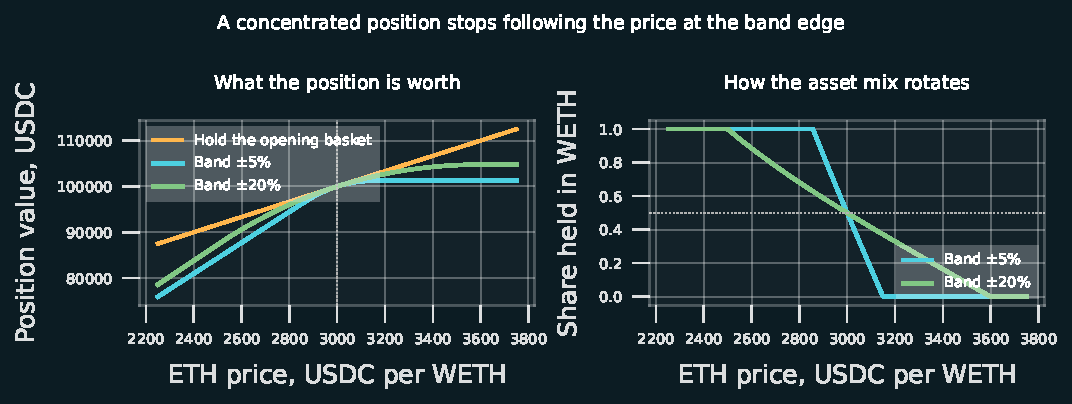
\includegraphics[width=0.92\linewidth]{figures/position_payoff.pdf}
\caption{A concentrated position versus a passive holding of the same opening
basket. Left: the position tracks the basket while the price sits inside the
band and stops following it at the edges, so it gives up the upside of a rally
while keeping the downside of a fall. Right: the asset mix rotates from WETH
to USDC as the price rises and freezes at the edge. Illustrative parameters:
\usdc{100000} entered at \SI{3000}{USDC} per WETH.}
\label{fig:payoff}
\end{figure}

\subsection{Two losses, one larger}

Impermanent loss (IL) is the shortfall of the position against holding the
initial deposit. For a full-range position with equally valued legs and price
ratio $r=q_t/q_0$,
\begin{equation}
\mathrm{IL}(r) = \frac{2\sqrt{r}}{1+r} - 1,
\label{eq:il}
\end{equation}
which is second order in the price move; at $r=1.2$ it is $-0.41\,\%$. On v3
the same expression applies only inside the band, and outside it the position
is a one-sided holding, so IL depends on where the band was
placed\cite{loesch2021impermanent}.

LVR is sharper. Compare the position with a portfolio that continuously
rebalances to hold the same instantaneous exposure. A second-order expansion of
the full-range value shows that the LP falls behind that portfolio at the rate
\begin{equation}
\mathrm{dLVR}_t = \frac{1}{8}\,\sigma^2\,V_t\,\mathrm{d}t,
\label{eq:lvr}
\end{equation}
the loss-versus-rebalancing of Milionis et al.\cite{milionis2022lvr}. Adverse
selection therefore grows with the square of volatility and with position size,
and fee income must exceed it for passive provision to be viable. Concentration
raises fee density but not the fee rate, so it helps only when the extra fee
share outweighs the extra exposure to arbitrage; Section~\ref{sec:related}
finds that on many large pools it does not. Figure~\ref{fig:losses} shows the
shape of both losses.

\begin{figure}[tbp]
\centering
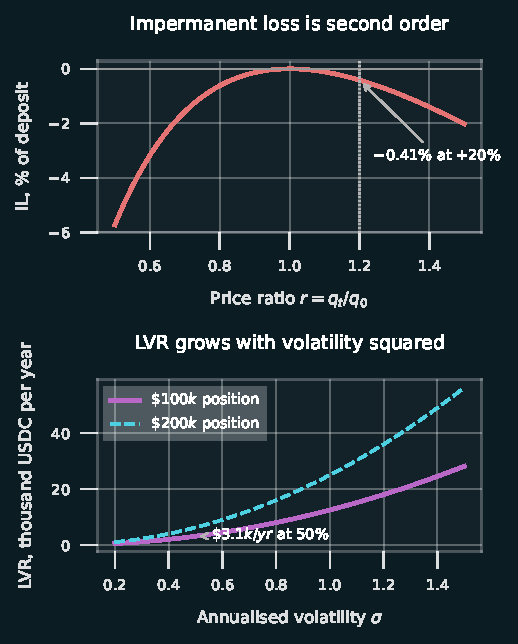
\includegraphics[width=0.55\linewidth]{figures/il_lvr.pdf}
\caption{The two losses. Top: impermanent loss against the price move, second
order and small for a full-range position. Bottom: the LVR rate against
volatility for a \usdc{100000} and a \usdc{200000} position, showing both the
quadratic dependence on volatility and the linear dependence on size.}
\label{fig:losses}
\end{figure}

\subsection{The decisions and the risk}

An LP that wants to improve on the passive outcome must decide when to act,
where and how wide to place the next band, and how much market risk to carry.
The levers interfere, and Table~\ref{tab:levers} states what each one buys and
what it costs. Because acting is lumpy, the problem is one of impulse
control\cite{anchuri2026rammstein}, and because the outcome is uncertain the
right measure is profit per unit of risk. We use the annualised Sharpe ratio
and the conditional value-at-risk (CVaR) at the $5\,\%$ level as primary
statistics; CVaR is coherent and has a convex representation that can be
optimised directly\cite{rockafellar2000cvar}. Figure~\ref{fig:decisions} makes
the sequence of decisions and costs concrete.

\begin{table}[tbp]
\caption{The three levers and the trade-off each carries. Every return in the
study is measured after the costs of the active levers are charged: the
liquidity leg pays gas, slippage and impermanent loss, and the hedge leg adds
funding and perp fees once the overlay is enabled.}
\label{tab:levers}
\centering
\small
\begin{tabular}{@{}L{0.16\linewidth}L{0.20\linewidth}L{0.25\linewidth}L{0.27\linewidth}@{}}
\toprule
\textbf{Lever} & \textbf{Choice} & \textbf{Buys} & \textbf{Costs} \\
\midrule
Timing $\kappa_t$ & hold or recenter & fee income on a band close to the price & gas and slippage; the fee position restarts \\
Width $w_t$ & width of the band, in tick spacings & fee density for a given deposit & time until the price reaches an edge \\
Hedge $h_t$ & short fraction of ETH delta & removal of directional swings & funding and perp trading fees \\
\bottomrule
\end{tabular}
\end{table}

\begin{figure}[tbp]
\centering
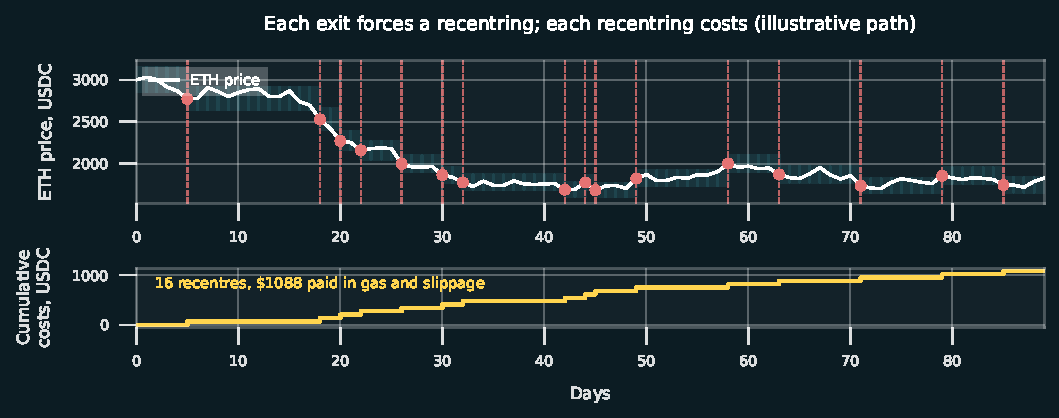
\includegraphics[width=0.92\linewidth]{figures/decision_path.pdf}
\caption{Why acting is a decision rather than a rule. An illustrative price
path with a $\pm5\%$ band: each exit forces a recentring, and each recentring
adds gas and slippage to a cost that only ever grows. The path is illustrative
and the costs are simplified; the study charges per-block gas and slippage on
the inventory actually swapped.}
\label{fig:decisions}
\end{figure}

\section{Related Work}
\label{sec:related}

The economics of passive provision is now well understood. Milionis et al.\
formalised the loss a constant-product LP suffers against a delta-rebalanced
portfolio and derived the rate $\frac{1}{8}\sigma^2 V$ for a full-range
position; the loss appears on any price path, informed traders or not, and
protocol fees and the choice of curve shift only the balance\cite{milionis2022lvr}.
Fritsch and Canidio measured the losses on real pools and found that arbitrage
losses typically dominate the fees earned, with passive full-range positions
outperforming concentrated ones in their sample\cite{fritsch2024measuring}.
Loesch et al.\ studied v3 positions directly and showed that concentration
magnifies impermanent loss when the price leaves the band\cite{loesch2021impermanent}.
Together these results define the terrain: gross fee yield is not an LP's
return.

A second line of work learns the LP's decisions. Zhang et al.\ train a hedged
double deep Q-network and report large gains over baselines, but the hedge is
assumed frictionless and the policy sees no regime
features\cite{zhang2023adaptive}. A recent replication replaces the feature
extractor of that model with a sequence model and a revised reward, and adds
two baselines; it keeps the simulated setting and reports no statistic that
adjusts for risk\cite{zhang2025mamba}. ZeroSwap learns the spread of a market maker so
that quoted prices track an external reference, an orthogonal lever to range
placement\cite{nadkarni2023zeroswap}. RAmmStein poses regime-dependent
rebalancing thresholds as a problem of impulse control and reports that
rebalancing lazily when the regime warrants it improves net ROI with far fewer
rebalances, though its net metric excludes impermanent loss and the study
relies on off-chain data for one pair\cite{anchuri2026rammstein}. Chionas et
al.\ treat concentrated liquidity as a risk-aversion problem in simulation and
find that higher volatility and gas widen optimal positions and reduce
rebalancing, while a risk penalty trims the adverse tail; their analysis uses
no on-chain data and no hedge\cite{chionas2026concentrated}. Classical market
making supplies the risk-sensitive vocabulary we use, but its state is a limit
order book and its actions are quotes, not range geometry\cite{avellaneda2008high}.

The closest study to this report trains a PPO agent on hourly WETH/USDC
$0.05\,\%$ data from the same primary pool used here\cite{xu2025defi}. Xu and
Brini let the policy decide when to redeploy and how wide to keep the band,
penalise the loss-versus-rebalancing rate inside the reward, and compare the
learned policy with a periodic reset across eleven rolling windows; the active
policy wins seven of them. Three differences matter for the claims of this
report. Their agent carries no hedge, so directional risk stays in the
position. Market outcomes are simulated from closed-form fee and loss
expressions at hourly resolution, with a fixed gas charge and no slippage,
rather than replayed from the recorded events. And the evaluation is thinner:
performance is reported as cumulative reward, without a statistic that adjusts
for risk or an uncertainty interval, and the best of fifty trained agents is
selected for each window.

The learning machinery is standard. We use proximal policy optimisation with
clipping (PPO)\cite{schulman2017ppo}, implemented through Stable-Baselines3 on
Gymnasium environments\cite{raffin2021stablebaselines3,towers2024gymnasium},
and evaluate risk with CVaR at the $5\,\%$ level through its
Rockafellar--Uryasev representation\cite{rockafellar2000cvar}.

No study surveyed here combines the parts this report tests. The line that
learns decisions supplies them only in pieces: a hedge learned without
friction, a range policy learned without the hedge, and a mean metric rather
than one that adjusts for risk. Two of the answers here are measured rather
than assumed. The passive benchmarks are decomposed into fees, impermanent
loss, gas and slippage on both fee tiers, so the economics answer rests on the
pools of this study rather than on a survey, and the ways a standard policy
collapses on the task are reported as a result rather than hidden in an
implementation note.

What remains is the combination studied here. One risk-sensitive policy
chooses timing, width and hedge. A cost ledger replayed from the tape,
bounded against an exact integer engine, prices every friction on both legs.
Sharpe and tail statistics carry paired intervals across seeds. And a boundary
states where active management stops paying. The rest of the report tests that
combination, with the hedge leg the one part still pending: the overlay is
disabled in the shipped configuration, so the hedge results are marked as such.

\section{The Liquidity Provider's Decision Problem}
\label{sec:formulation}

We model the LP's problem as a risk-sensitive Markov decision process with
impulse control. Decisions are taken every ten minutes over an episode of
thirty days. At each decision the agent sees a fixed observation, chooses
between holding and acting, and receives a reward that measures how far the
strategy's value has moved beyond a passive benchmark, net of every cost. The
volatility regime and order flow are latent, so the process is partially
observed: the agent sees only the history summarised in the observation.
Figure~\ref{fig:loop} shows one decision cycle.

\begin{figure}[tbp]
\centering
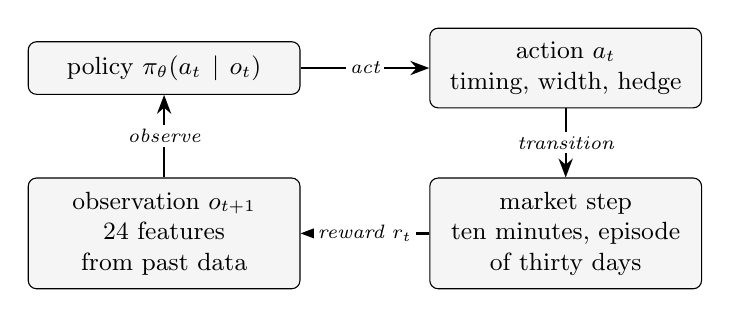
\begin{tikzpicture}[
  font=\small,
  box/.style={draw, rounded corners=3pt, align=center, inner sep=5pt,
              fill=black!4, text width=3.1cm},
  arr/.style={-{Stealth[length=2.4mm]}, thick},
  lbl/.style={font=\scriptsize\itshape, midway, fill=white, inner sep=1.5pt}
]
  \node[box] (policy) at (0,2.1) {policy $\pi_\theta(a_t \mid o_t)$};
  \node[box] (action) at (5.1,2.1) {action $a_t$\\timing, width, hedge};
  \node[box] (market) at (5.1,0) {market step\\ten minutes, episode of thirty days};
  \node[box] (obs)    at (0,0)   {observation $o_{t+1}$\\24 features from past data};
  \draw[arr] (policy) -- node[lbl] {act} (action);
  \draw[arr] (action) -- node[lbl] {transition} (market);
  \draw[arr] (market) -- node[lbl] {reward $r_t$} (obs);
  \draw[arr] (obs) -- node[lbl] {observe} (policy);
\end{tikzpicture}
\caption{One cycle of the LP decision process. The policy acts every ten
minutes; a decision to rebalance moves the band and charges gas and slippage,
while a decision to hold leaves the position where it is. Rewards accumulate
over an episode of thirty days against the fixed opening basket.}
\label{fig:loop}
\end{figure}

\subsection{State}

The observation contains 24 features, all computed from information available
at the decision time. Table~\ref{tab:observation} groups them by source. The
band geometry deserves emphasis: the action space is written in tick spacings
relative to the current tick, so a policy that cannot see how close the price
is to an edge cannot time a rebalance at all. Heavy-tailed features such as
price, liquidity and gas are compressed with a signed logarithm so that every
dimension reaches the network on the same scale.

\begin{table}[tbp]
\caption{The 24 observation features, grouped by source. Every field is
computed from information available at the decision time, so an observation at
time $t$ cannot contain a bar from $t+1$.}
\label{tab:observation}
\centering
\small
\begin{tabular}{@{}L{0.18\linewidth}L{0.65\linewidth}r@{}}
\toprule
\textbf{Group} & \textbf{Features} & \textbf{n} \\
\midrule
Market & price, sqrt price, tick, 1\,h and 24\,h log returns, realised 24\,h volatility & 6 \\
Position & in-range flag, position value, two uncollected fee balances, IL against the fixed basket & 5 \\
Pool & active liquidity, fee tier & 2 \\
Costs & recent gas price, recent ETH reference price & 2 \\
Regime & regime label (bull, bear, sideways, high volatility) & 1 \\
Time & step in episode, steps remaining & 2 \\
Band & distance to each band edge and band width, in tick spacings & 3 \\
Hedge & short ratio, hedge equity, recent funding rate & 3 \\
\midrule
 & \textbf{Total} & \textbf{24} \\
\bottomrule
\end{tabular}
\end{table}

\subsection{Action}

At each decision the agent selects a factored action
\begin{equation}
a_t = (\kappa_t,\, c_t,\, w_t,\, h_t),
\label{eq:action}
\end{equation}
whose four heads are described in Table~\ref{tab:action}. On the $0.05\,\%$
primary pool the liquidity head alone has $1+9\times10=91$ options. The
shipped configuration learns the liquidity head with the hedge overlay
disabled; when the overlay is enabled its ratio is set by configuration.
Promoting $h_t$ to a learned head, and the hedge-leg benchmarks, are planned
for the last two questions and their results remain pending.

\begin{table}[tbp]
\caption{The four action heads. Widths are given as half the band width, in
tick spacings. The primary pool's spacing of $10$ uses all ten widths; the
contrast pool's spacing of $60$ uses the six-width ladder.}
\label{tab:action}
\centering
\small
\begin{tabular}{@{}L{0.14\linewidth}cL{0.28\linewidth}L{0.41\linewidth}@{}}
\toprule
\textbf{Head} & \textbf{Symbol} & \textbf{Options} & \textbf{Meaning} \\
\midrule
Rebalance & $\kappa_t$ & hold, act & spend gas and slippage to move the band, or leave it \\
Centre & $c_t$ & $-4,\dots,4$ spacings & shift the centre of the new band around the current tick \\
Width & $w_t$ & $\{1,2,5,10,25,50,$\newline $100,250,500,1000\}$ spacings & half of the new band's width \\
Hedge & $h_t$ & $\{0,0.25,0.5,0.75,1.0\}$ & fraction of the LP's ETH delta carried by the short \\
\bottomrule
\end{tabular}
\end{table}

\subsection{Reward}

A rebalance converts inventory and pays for the privilege. Writing $V_t$ for the
position value, $H_t$ for the fixed value of the opening deposit held
passively, and the hedge cash flows as mark PnL $\pi_t$, funding $\phi_t$ and
perp cost $\tau_t\le 0$, the reward is
\begin{align}
r_t = \frac{1}{W_0}\Big(
  & \mathrm{fees}_t - \mathrm{gas}_t - \mathrm{slip}_t
    + \Delta(V_t - H_t) \notag \\
  & + \pi_t + \phi_t + \tau_t - \lambda\,\hat\sigma_t \Big),
\label{eq:reward}
\end{align}
whose terms are defined in Table~\ref{tab:reward}. Dividing by the initial
capital $W_0$ keeps value targets at a workable scale without hiding any cost.
The excess is measured against the \emph{fixed} opening basket: $H_t$ is never
rebased at a rebalance, so the episode sum equals the excess over holding that
basket, which is the quantity the evaluation reports.

\begin{table}[tbp]
\caption{Every term of the reward, in token0 (USDC) units before the $1/W_0$
scaling. Gas and slippage enter as positive magnitudes and carry a minus sign
in the reward.}
\label{tab:reward}
\centering
\small
\begin{tabular}{@{}L{0.16\linewidth}L{0.62\linewidth}c@{}}
\toprule
\textbf{Term} & \textbf{Meaning} & \textbf{Sign} \\
\midrule
$\mathrm{fees}_t$ & fee income earned in the step & $+$ \\
$\mathrm{gas}_t$ & gas for mints, burns, collects and rebalancing swaps & $-$ \\
$\mathrm{slip}_t$ & slippage on the inventory actually swapped & $-$ \\
$\Delta(V_t-H_t)$ & change in position value against the fixed opening basket & $\pm$ \\
$\pi_t$ & mark PnL of the short perpetual & $\pm$ \\
$\phi_t$ & funding paid or received on the short & $\pm$ \\
$\tau_t$ & perp taker cost of adjusting the short & $\le 0$ \\
$\lambda\,\hat\sigma_t$ & penalty on recent reward volatility, $\lambda=0$ by default & $-$ \\
\bottomrule
\end{tabular}
\end{table}

\subsection{Risk and benchmarks}

The learning objective is the discounted return with a penalty on recent
reward volatility: the risk term in Eq.~\eqref{eq:reward} subtracts a multiple
of the trailing standard deviation of per-step equity changes, with $\lambda=0$
by default. Tail risk is measured in the evaluation instead. With losses $L=-G$
defined on the episode return $G$, the conditional value-at-risk at level
$\alpha$ is
\begin{equation}
\mathrm{CVaR}_\alpha(L) = \min_{\nu\in\mathbb{R}}
\left\{\nu+\frac{1}{1-\alpha}\mathbb{E}\big[(L-\nu)^+\big]\right\},
\label{eq:cvar}
\end{equation}
the Rockafellar--Uryasev representation\cite{rockafellar2000cvar}, which we
report at $\alpha=0.95$. Evaluation therefore reports the annualised Sharpe
ratio and CVaR at $5\,\%$ as primary statistics, with raw PnL and excess over
HODL as secondary ones. Comparisons use paired per-window differences and
confidence intervals across seeds.

The hedge is a short perpetual position sized as a fraction of the LP's delta.
Its mark PnL over a step is the negative product of the short notional and the
price change, plus funding and the taker cost of adjusting the position. Three
reference points make the hedge leg interpretable: the unhedged LP, the
deterministic overlay, and a hedged HODL portfolio with matched beta. The last
is the benchmark that prevents us from declaring success against a weaker
opponent: a policy that merely removes directional risk must still beat a
passive portfolio with the same risk profile. The overlay is disabled in the
shipped configuration, so the hedged benchmark of
Table~\ref{tab:benchmarks} remains pending.

\section{The Undertow Testbed}
\label{sec:system}

Answering C1--C4 requires an instrument, not an argument. Undertow is that
instrument: a testbed with two engines in which the same policy can be trained
cheaply and then measured against exact accounting on real on-chain events.
Figure~\ref{fig:system} sketches the data flow; this section describes each
stage and, just as importantly, the failure modes the testbed was built to
survive.

\begin{figure}[t]
\centering
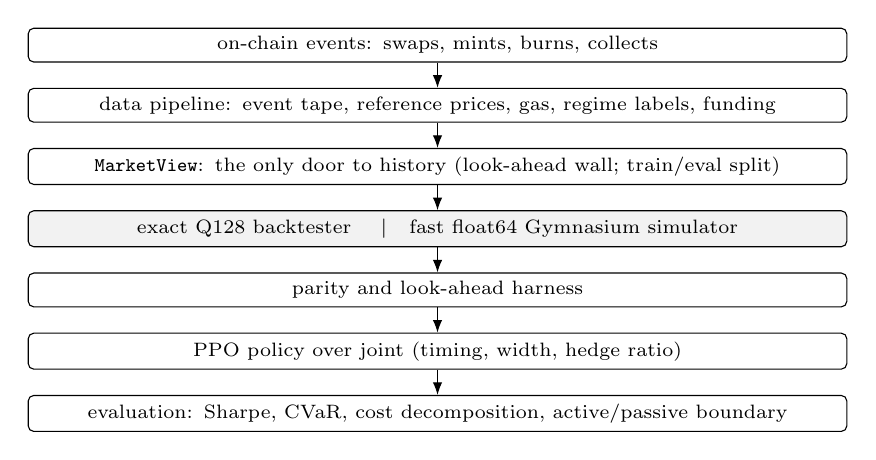
\begin{tikzpicture}[
  font=\scriptsize,
  box/.style={draw, rounded corners=2pt, align=center, inner sep=3pt,
              text width=0.84\columnwidth},
  >={Latex[length=1.6mm]},
  node distance=3.2mm,
]
\node[box] (events) {on-chain events: swaps, mints, burns, collects};
\node[box, below=of events] (pipe) {data pipeline: event tape, reference prices, gas, regime labels, funding};
\node[box, below=of pipe] (view) {\texttt{MarketView}: the only door to history (look-ahead wall; train/eval split)};
\node[box, below=of view, fill=black!5] (engines) {exact Q128 backtester \quad\textbar\quad fast float64 Gymnasium simulator};
\node[box, below=of engines] (parity) {parity and look-ahead harness};
\node[box, below=of parity] (rl) {PPO policy over joint (timing, width, hedge ratio)};
\node[box, below=of rl] (eval) {evaluation: Sharpe, CVaR, cost decomposition, active/passive boundary};
\draw[->] (events) -- (pipe);
\draw[->] (pipe) -- (view);
\draw[->] (view) -- (engines);
\draw[->] (engines) -- (parity);
\draw[->] (parity) -- (rl);
\draw[->] (rl) -- (eval);
\end{tikzpicture}
\caption{Undertow: from on-chain events to a risk-sensitive policy. The two
engines share one \texttt{MarketView} and are reconciled by the parity harness
before any training result is reported.}
\label{fig:system}
\end{figure}

\subsection{Data: an on-chain event tape}

The data layer ingests the raw logs of two real USDC/WETH pools, the
$0.05\,\%$ primary study pool (\texttt{0x88e6a0\ldots f5640}, tick spacing
$10$) and the $0.30\,\%$ contrast pool (\texttt{0x8ad599\ldots e6d8}, spacing
$60$), and converts them into a single \emph{event tape} ordered by block and
containing swaps, mints, burns and collect events. Alongside the tape it
builds three auxiliary feeds: reference price closes at a resolution of one
minute, gas prices at each block, and regime labels produced by thresholds
committed in advance in the data module. A fourth feed, funding, is pulled from the Binance
perpetual market margined in USDT at its native $8\,\mathrm{h}$ cadence and
used by the hedge leg. The pinned window is \textbf{2022-01-01 to 2024-12-31
UTC}; the walk-forward split trains on 2022--2023 and evaluates on 2024, so the
test year is never seen during training or calibration. The primary pool's
training lane alone carries roughly $4.86\times 10^{6}$ events, which is why
the throughput work described below is a necessity rather than an optimization.

Two design rules protect the results. First, the tape is the ground truth:
prices, liquidity events and fees are the recorded on-chain values, not a
fitted process. Second, all access goes through \texttt{MarketView}, which
enforces both the block ordering and the train/eval boundary, so an
observation at time $t$ cannot read a bar from $t+1$ even by accident.

\subsection{The exact backtester}

The backtester replays a frozen policy against the tape using integer
arithmetic. Fee accrual is computed in Q128 fixed point from the pool's
recorded fee growth accumulators, exactly as the protocol does; liquidity
events update an external tick lattice seeded from a boundary snapshot, and
swap crossings are apportioned piecewise across the ticks they cross. The
resulting ledger satisfies an accounting identity by construction,
\begin{equation}
\texttt{net} = \texttt{fees} + \texttt{il} - \texttt{gas} - \texttt{slippage}
= \texttt{excess\_vs\_hodl},
\label{eq:ledger}
\end{equation}
with impermanent loss measured against the fixed initial deposit basket. The
policy protocol exposes no learning method, since a backtested policy is frozen
by construction, and every ledger records the config hash, seed and git commit
that produced it.

\subsection{The fast simulator}

Training on the exact engine is infeasible at millions of steps, so the
simulator mirrors the same economics in float64. Its agent is
\emph{marginal}: agent liquidity never moves the price path, and the fee share
is $\ell_{\text{agent}} / (\ell_{\text{agent}} + \ell_{\text{pool}})$ evaluated
against the tape's recorded active liquidity. The tick lattice supports both
minted agent positions and the external pool lattice, and the bookkeeping of
snapshots and the tape path uses exact Python integers so that a large gross
liquidity residue cannot silently corrupt a small delta, while a
burn larger than the position still raises. Two price modes share one
interface: \emph{replay}, which walks the reference closes at a resolution of
one minute, and a jump diffusion whose latent regimes follow a Markov chain
with four states anchored to the regime labels, with drift and volatility for
each state, Student-$t$ jumps, and transitions estimated from the training
split only. A throughput pass replaced
scans at each step with indexes computed as of that step, cached the lattice
keys and window views, and moved the vectorised environments into separate
processes; on the pinned hardware the PPO throughput of the full pipeline rose
from roughly $150$--$175$ to about $450$ steps per second. Actions execute at
the decision price observed \emph{before} the interval advances, matching the
backtester and the latency a live LP would face.

\subsection{Parity and look-ahead}

Two numeric worlds are only useful if their disagreement is bounded. The parity
harness feeds the simulator and the backtester the same price path, positions
and gas series and compares fees, impermanent loss and PnL under a stated
relative tolerance ($10^{-3}$ for float64 against exact integers). After the
fee engine was made exact, the remaining drift on the replay of real data is
small: mean fee differences within each seed are on the order of $10^{-7}$ of
notional, and impermanent loss matches exactly, comfortably inside tolerance.
The harness originally exercised only the HOLD policy, which never rebalances;
it now also runs a policy that rebalances, which is precisely the path the
C1--C3 fees depend on. Alongside parity, a suite of look-ahead probes attacks
the composed system: each component is checked to raise rather than read the
future, and the probes include deliberately adversarial windows at the
train/eval seam.

\subsection{Learning and the failure modes it survived}

The learning setup is deliberately modest: PPO with clipping on a $2\times256$
MLP, discount $0.99$, generalized advantage estimation (GAE) with
$\lambda = 0.95$, clip $0.15$, five fixed seeds, and one million timesteps per
seed. That simplicity is a feature: if a plain PPO cannot learn the task, the
task or the interface is broken, and it was. The first two runs collapsed
instead. Each seed locked onto one deterministic action, some always holding
and some always repeating a single rebalance, and the measured advantage did
not separate the actions, with a correlation across actions near zero.
Diagnosing that collapse produced three interface fixes that are now part of
the testbed and are ablated for C2. The observation gained the three band
geometry features, and the features with heavy tails gained signed log
compression. The reward term for impermanent loss was moved from a rolling
entry basket to the fixed initial HODL basket so that the reward at each step
equals the change in the reported excess metric; the old parity harness could not
catch that divergence because it only ran HOLD. Episodes gained window
resampling: a reset without an episode seed now advances to a new window of
30 days instead of replaying the same lane for a million steps. Two cost defects were
fixed on the way: rebalance slippage is charged on the inventory imbalance
actually swapped rather than the whole position value, and the marginal fee
credit is capped at the augmented denominator share so that a tiny agent
cannot claim an outsized fee fraction. Each fix ships with a unit test and a
decision record; the C2 table in Section~\ref{sec:results} lists symptom,
diagnosis, fix and evidence.

\subsection{Evaluation and reproducibility}

The evaluation runner freezes a checkpoint and scores it on windows held out
from training, emitting each episode's equity curve, cost ledgers and regime
slices, then aggregating annualized Sharpe, raw PnL and excess-versus-HODL with
confidence intervals across seeds and regimes. \pending{CVaR at $5\,\%$ exists
as a metric in the metrics layer; wiring it into the aggregated evaluation
report is the S21 deliverable, after which it joins the primary statistics.}
The RQ1 ablation table, the RQ2 regime matrix and the report on the gap
between simulator and backtester are generated from the same runner, and a
dashboard that is read only replays policies against price and ranks runs by
Sharpe out of sample. Every artefact carries the config hash and commit, so a
reported number can be traced to the exact run that produced it.

\section{Experimental Design}
\label{sec:design}

The claims of Section~\ref{sec:intro} are only as credible as the protocol that
tests them, so the protocol is fixed before any result is inspected, following
the binding measurement protocol of ADR-030.

\subsection{Data, windows and episodes}

The study uses two real USDC/WETH pools: the $0.05\,\%$ primary pool (spacing
$10$) and the $0.30\,\%$ contrast pool (spacing $60$). The study period runs
from 2022-01-01 to 2024-12-31 (UTC) and is divided walk-forward: 2022--2023
supplies the training data and 2024 is held out for evaluation. Training
episodes are windows of 30 days sampled from the training split with the
environment's window resampling; evaluation tiles the 2024 split into
nonoverlapping windows of 30 days (thirteen windows, the last partial), and no
episode crosses the split boundary. Each episode runs at a decision cadence of
10 minutes with \usdc{100000} of agent capital, which keeps the agent marginal
relative to pool liquidity and the fee share assumption honest. Every
configuration in the study is trained with the five fixed seeds
$\{0,1,2,3,4\}$ and one million timesteps per seed.

\subsection{Benchmarks}

A learned policy that beats only the weakest rule written by hand has
demonstrated nothing. Our benchmark ladder therefore includes the full
family of six policies, two additional reference points, and the hedged HODL
benchmark matched in beta described in Section~\ref{sec:formulation}.
Table~\ref{tab:benchmarks} lists them. The \emph{best static width} is selected
on the training split and then frozen for evaluation, so it represents a
heuristic with hindsight over the training period but not over the test period.

\begin{table}[t]
\caption{Benchmark policies. Each row is a frozen rule; the learned policy is
compared against all of them, and C3 is claimed only if it beats the best
static width and the hedged HODL matched in beta, not just \textsf{hodl}.}
\label{tab:benchmarks}
\centering
\small
\begin{tabular}{@{}p{0.28\columnwidth}p{0.64\columnwidth}@{}}
\toprule
\textbf{Benchmark} & \textbf{Rule} \\
\midrule
\textsf{hodl} & Hold the initial token mix; never provide liquidity. \\
\textsf{passive\_narrow} & Deploy a $\pm 5\,\%$ band once; never recenter. \\
\textsf{passive\_wide} & Deploy a $\pm 20\,\%$ band once; never recenter. \\
\textsf{full\_range\_v2} & Full range, equivalent to Uniswap~v2. \\
\textsf{tau\_reset} & Recenter whenever the price exits the live band. \\
\textsf{cost\_aware} & Recenter at most daily, and only when the estimated fee gain exceeds gas. \\
Best static width & The ladder width with the best Sharpe on the training split, frozen for test. \\
Hedged HODL & Initial basket plus a short perp matched to its beta, with funding and perp costs. \\
Learned policy & PPO over the joint (timing, width, hedge ratio) action space. \\
\bottomrule
\end{tabular}
\end{table}

\subsection{Metrics}

The two primary statistics are:
\begin{itemize}
  \item \textbf{Annualized Sharpe ratio.} For each episode, computed on the
  equity curve at the decision cadence and annualized with the
  $\sqrt{\text{periods}}$ rule at $52{,}596$ periods per year. We report the
  mean and a paired bootstrap confidence interval across seeds and windows.
  \item \textbf{CVaR at $5\,\%$.} The average of the worst $5\,\%$ of episode
  returns, pooled across seeds, with a bootstrap confidence interval. Because
  the tail is thin at 13 windows $\times$ 5 seeds, we also report the worst
  window and its decomposition.
\end{itemize}
Secondary statistics are raw PnL, excess-versus-HODL, annualized return,
Sortino ratio, maximum drawdown, rebalance count, and the cost ledger
(fee income, gas, slippage, realized impermanent loss). Every performance table
reports both layers, and tables for each regime stratify by the dominant regime
label of the window (bull, bear, sideways, high volatility). All comparisons
against a benchmark use paired differences within each window, so market moves
common to both policies do not inflate the apparent effect.

\subsection{Ablations}

The failure modes of C2 are ablated one at a time: band geometry removed from
the observation; training windows held fixed instead of resampled; the hedge
disabled; the reward's risk penalty toggled ($\lambda = 0$ versus
$\lambda > 0$); regime features removed. The C1 economic decomposition is
ablated over frictions (full model, no gas, static fee, no impermanent loss)
and repeated on the $0.30\,\%$ pool to test the prediction that a higher fee
tier buys a longer viable range. For C4 the runner sweeps the environment along
the axes that the economics identifies: realized volatility, volume relative to
liquidity, fee tier, gas price and capital. Each sweep point is evaluated on
replayed windows, so the boundary is measured against real market states rather
than a fitted process.

\subsection{Hypotheses and decision rules}

\begin{itemize}
  \item \textbf{C1 (limits).} The decomposition of the best passive benchmark
  is negative in excess-versus-HODL terms and dominated by adverse selection;
  we report where the sign flips across regimes and fee tiers.
  \item \textbf{C2 (failure modes).} Each ablated fix degrades the learned
  policy relative to the full interface, or reproduces on at least one seed
  the degenerate behavior documented in ADR-030, in which the policy repeats
  one action. The claim is descriptive: we report the failure, the diagnosis
  and the effect of the fix.
  \item \textbf{C3 (joint policy).} The learned policy's mean Sharpe exceeds
  the best static width's and the hedged HODL benchmark's, with a paired
  $95\,\%$ confidence interval excluding zero; its $5\,\%$ CVaR is no worse
  than the best heuristic's; and its action distribution is not degenerate
  across seeds.
  \item \textbf{C4 (boundary).} We report the fitted boundary of
  $\text{Sharpe}_{\text{learned}} - \text{Sharpe}_{\text{passive}} = 0$ along
  each environmental axis, with the analytical LVR threshold from
  Eq.~\eqref{eq:lvr} overlaid as the theoretical comparison.
\end{itemize}
Rules stated in advance are the point: they prevent the result from being
chosen after the fact. Where the evidence turns out negative, the negative
result is reported as the finding.

\subsection{Reproducibility}

Every training run writes a manifest with its config hash, git commit, seed
and library versions; every evaluation writes each episode's equity curve, cost
ledger and decision log. Determinism is enforced at the level of individual
components (seeded generators everywhere, no clock time in state) and
exercised by the parity and look-ahead suites. Running a reported
configuration again is expected to reproduce its learning curve, and a
reported number without a manifest behind it is treated as a bug.

\section{Results}
\label{sec:results}

\pending{This section is intentionally a stub while the RL experiments across
seeds run. It will report C1--C4 in order, and every number will come from the
locked runs (manifests under \texttt{results/}), never from a draft memory.
Nothing in this section may be filled until the runs complete.}

\subsection{C1: Where fees fail to cover LVR and rebalancing}
\pending{Report the passive benchmark cost decomposition (fees, impermanent
loss, LVR, gas, slippage) on both fee tiers, the cost of greedy versus lazy
rebalancing, and the sign of excess-versus-HODL across regimes. The
preliminary diagnostic over 15 windows recorded in ADR-030 motivates the
claim; the final table replaces it.}

\subsection{C2: Failure modes in naive RL}
\pending{Report the collapse before the fixes (policies that repeat one action,
flat learning curves) and the ablations of each fix (band geometry off, fixed
training window, reward measured against the rolling basket, execution at
decision time off), with the evidence for each diagnosis.}

\subsection{C3: The learned joint policy}
\pending{Report Sharpe and CVaR out of sample for the learned policy against
the full benchmark ladder of Table~\ref{tab:benchmarks}, paired within windows
and across seeds, plus the action distribution that shows the policy is not
degenerate and its decision boundaries recover the band exit and the trade-off
between fees and gas.}

\subsection{C4: The active/passive boundary}
\pending{Report the swept boundary where the learned and passive Sharpe
ratios are equal, as a function of volatility, volume relative to liquidity,
fee tier, gas and capital, with the analytical LVR threshold from
Eq.~\eqref{eq:lvr} overlaid.}

\section{Discussion}
\label{sec:discussion}

\pending{The interpretive discussion is deferred until the locked runs land: it
will connect the four answers to the active/passive boundary and to the design
lessons for learning in this setting. The validity concerns below do not depend
on the results.}

The simulator replays recorded events, so prices, liquidity and fee growth are
real rather than modelled. Its marginal-agent assumption is the main
simplification: the position never moves the price, and its fee share is
proportional to active liquidity. That is the standard replay assumption and it
is recorded with every run, but it cannot capture queueing at the tick level or
the impact of an unusually large position. The gas model charges representative
per-action units rather than per-transaction receipts, so gas is a defensible
floor rather than an exact quote, and the hedge uses a perpetual proxy whose
funding and basis are representative rather than exact for a specific venue.

Several threats bound what the study can claim. The evidence covers one asset
pair at two fee tiers, so the boundary is measured within that scope and does
not automatically transfer to other pairs. CVaR at $5\,\%$ averages a handful of
episodes, so it is reported with bootstrap intervals and the worst window rather
than treated as decisive on its own. The regime labels come from thresholds
fixed in advance; they organise the reporting and anchor the training process,
but they are a labelling device, not a discovered state. The boundary sweep
compares several axes at once, so paired intervals on a pre-registered primary
metric carry the inference, and any secondary win is labelled as such.

The parity check bounds the distance between the simulator and the backtester,
not the distance between the backtester and reality. Where the data allow, the
external part of the gap is quantified by reconciling fees and collects; where
they do not, latency, order-flow privacy and MEV are discussed rather than
measured. We therefore claim results about performance under risk on recorded
market states under a stated cost model. We do not claim deployable
profitability, optimality of the action grid, or that the policy would survive
market conditions absent from 2022 to 2024.

\section{Conclusion}
\label{sec:conclusion}

The story began with a simple bargain: concentrate liquidity in a price range,
earn more fees while the price stays inside it. The bargain hides a cost. The
same position that earns the fees is the position that loses to informed order
flow, and on real pools that loss can exceed the income. An LP who wants to do
better than accept it must decide when to recenter, how wide to stay and how
much risk to hedge, and each decision is expensive and uncertain.

This report set out to measure whether a risk-sensitive learned policy can make
those decisions jointly better than the best rules written by hand, and to find
where active management stops paying. Answering that required a world in which
costs are measured rather than assumed, so we built a testbed from two years of
recorded trades, with an exact replay engine for ground truth and a classical
simulator for training, reconciled by a parity harness. The study then asked
four questions: where fees fail, why a standard agent fails, whether a learned
policy wins out of sample, and where the boundary between active and passive
provision lies.

\pending{This paragraph will close with the measured verdicts once the
experiments complete. Its shape is fixed: what the four answers were, which of
them held, and what the boundary looked like.}

The boundary of the study is also a map for future work. The action space can be
extended with continuous width and an explicit exit decision. The boundary sweep
can cover more pairs and fee tiers. Latency, private order flow and the exact
funding of a real venue can be modelled rather than proxied. Each extension is a
re-run of the same testbed rather than a redesign of it, which is the point of
building the testbed before asking the question.


\bibliographystyle{IEEEtran}
\bibliography{references}

\end{document}
